% Provenance (never printed): see sources/outline_sources.md (Year 1: stress and
% principal stresses in 2D; strain; pure and simple shear; elastic, brittle and ductile
% behaviour; the strength envelope of the lithosphere). Strength envelopes from
% figdata/bachelor-1/strength_envelope.py (Byerlee 1975; flow laws of Gleason and Tullis
% 1995 and Hirth and Kohlstedt 2003 as compiled by Lopez-Sanchez; geotherms of ch. 10);
% exercise and problem values in the Book 3 scratch calculator calc/ch16.py. Traction,
% shear stress, the stress and strain tensors, Hooke's law, Young's modulus and viscosity
% belong to the physics series and are recalled, never defined (sync 1 ruling).
\chapter{प्रतिबल, विकृति और रियोलॉजी}\label{ch:b1:stress-strain-rheology}

1960 के दशक में, डेनवर के निकट रॉकी माउंटेन आर्सेनल में एक निपटान-कूप में पंप किया गया अपशिष्ट द्रव, सतह से \qty{3.7}{km} और \qty{7.0}{km} नीचे की दरार-युक्त क्रिस्टलीय आधारशिला में फैल गया, और भूकंप आए। वे चट्टान के उस भाग के भीतर रहे जहाँ द्रव-दाब लगभग \qty{3.2}{MPa} से अधिक बढ़ गया था।
% ledger: hb81:denver
आधी सदी बाद वही बात ओकलाहोमा में बड़े पैमाने पर हुई, जहाँ तेल और गैस के साथ ऊपर लाया गया खारा पानी भूमि में वापस पंप किया जाता है। राज्य में और उसके आसपास, परिमाण 3 या अधिक के भूकंप 2005 से 2008 तक वर्ष में एक से पाँच थे, फिर 2009 में \num{20}, 2014 में \num{585} और 2015 में \num{888}, यानी प्रतिदिन दो से अधिक; परिमाण 5.7 और 5.8 के झटकों ने 2011 में प्राग को और 2016 में पॉनी को हिलाया। अकेले चार उच्च-आयतन निपटान-कूप संयुक्त राज्य के मध्य भाग के भूकंपों के एक-पाँचवें के लिए ज़िम्मेदार हो सकते हैं, और कुछ ने \qty{30}{km} से अधिक दूर भी झटके उत्पन्न किए।
% ledger: usgs:oklahoma-rate, usgs:prague-pawnee, keranen:oklahoma
जल कुछ भी नहीं हटाता; वह केवल चट्टान के छिद्रों में द्रव का दाब बढ़ाता है। एक भ्रंश को क्यों खिसकना चाहिए? उत्तर के लिए तीन विचार चाहिए, जो इस अध्याय का विषय हैं: चट्टान के भीतर एक तल पर प्रतिबल, वह शर्त जिसके तहत तल टूट जाता है, और यह तथ्य कि छिद्र-द्रव का दाब उन दो पक्षों को एक साथ दबाने वाले बल के विरुद्ध गिना जाता है। इन्हें, और गरम चट्टान के एक विसर्पण-नियम के साथ, हम पूरे \omterm{def:b1:layered-earth:lithosphere}{स्थलमंडल} की सामर्थ्य को गहराई के विरुद्ध खींच सकते हैं।

\begin{recall}
एक बल जो किसी सतह पर फैला है, प्रति इकाई क्षेत्र बल से कार्य करता है, पास्कल में; स्थिर द्रव में दाब गहराई के साथ $\rho g z$ के रूप में बढ़ता है (भौतिकी की पुस्तकें)। एक स्प्रिंग, और छोटे विरूपणों में एक ठोस, हुक के नियम का पालन करते हैं: विकृति प्रतिबल के समानुपाती है, यंग के मापांक के स्थिरांक के साथ; एक श्यान द्रव अपनी कर्तन-दर के समानुपाती रूप से विरोध करता है, जिसका स्थिरांक उसकी श्यानता है। भौतिकी की पुस्तकों का विश्वविद्यालय वर्ष 3 वाला खंड प्रतिबल और विकृति का त्रि-आयामी वर्णन टेंसरों से करता है; इस अध्याय को केवल दो चाहिए। एक सममित $2\times2$ आव्यूह के दो वास्तविक आइगेनमान और दो लंबवत आइगेनसदिश होते हैं (गणित, वर्ष 1)। \cref{ch:b1:heat-budget} के \omterm{def:b1:heat-budget:geotherm}{जियोथर्म} गहराई पर तापमान देते हैं; भ्रंशों से पुस्तक 1, कक्षा 7 में मिले थे।
\end{recall}

\section{दो आयामों में प्रतिबल}\label{sec:b1:stress-strain-rheology:stress}

किसी चट्टान को विचार में एक छोटी समतल सतह के साथ काटिए। सतह की एक ओर की चट्टान दूसरी पर एक बल लगाती है, और प्रति इकाई क्षेत्र बल उस सतह पर का ट्रैक्शन है, भौतिकी पुस्तकों के शब्द में। उसकी दिशा सामान्यतः सतह के अभिलंब की दिशा नहीं होती।

\begin{definition}[अभिलंब प्रतिबल]
\label{def:b1:stress-strain-rheology:stress}
किसी चट्टान के एक बिंदु से होकर एक तल पर, एक ओर की चट्टान दूसरी पर जो प्रति इकाई क्षेत्र बल लगाती है, उसका एक घटक तल के अभिलंब के अनुदिश है, \emph{अभिलंब प्रतिबल}\index{अभिलंब प्रतिबल} $\sigma_n$, और एक घटक तल के अनुदिश है, कर्तन-प्रतिबल $\tau$। पृथ्वी विज्ञानों में अभिलंब प्रतिबल तब धनात्मक गिना जाता है जब वह संपीड़न करे।
\end{definition}

यह चिह्न-परिपाटी इंजीनियर की परिपाटी के विपरीत है। इसे इसलिए चुना गया है क्योंकि ठोस पृथ्वी में लगभग हर प्रतिबल संपीड़न है: ऊपर की चट्टान का भार उसके नीचे की हर चीज़ को दबाता है।

हम एक ऊर्ध्वाधर तल में काम करते हैं, क्षैतिज अक्ष $x$ और एक अक्ष $y$ के साथ। $x$ के लंबवत तल पर \omterm{def:b1:stress-strain-rheology:stress}{अभिलंब प्रतिबल} $\sigma_{xx}$ है और कर्तन-प्रतिबल $\sigma_{xy}$; $y$ के लंबवत तल पर वे $\sigma_{yy}$ और $\sigma_{yx}$ हैं। दो कर्तन-प्रतिबल बराबर हैं: एक छोटे वर्ग पर, ऊर्ध्वाधर भुजाओं पर कर्तन-बल आघूर्ण $\sigma_{xy}a\cdot a$ का युग्म बनाते हैं, एक भुजा $a$ के लिए, क्षैतिज भुजाओं पर युग्म $\sigma_{yx}a\cdot a$ विपरीत दिशा में घूमता है, और यदि वे भिन्न होते तो वर्ग घूम जाता। अतः किसी बिंदु पर प्रतिबल तीन संख्याओं से वर्णित होता है, और वे हर तल पर उसे देने के लिए पर्याप्त हैं।

\begin{proposition}[झुके तल पर प्रतिबल]
\label{prop:b1:stress-strain-rheology:transformation}
मान लीजिए एक तल का इकाई अभिलंब $\vec n = (\cos\theta, \sin\theta)$ है, कोण $\theta$ पर, अक्ष $x$ से, और मान लीजिए $\vec m = (-\sin\theta, \cos\theta)$ तल के अनुदिश इकाई सदिश है। उस पर अभिलंब और कर्तन प्रतिबल हैं
\begin{align*}
  \sigma_n &= \sigma_{xx}\cos^2\theta + 2\sigma_{xy}\sin\theta\cos\theta + \sigma_{yy}\sin^2\theta
           = \frac{\sigma_{xx}+\sigma_{yy}}{2} + \frac{\sigma_{xx}-\sigma_{yy}}{2}\cos2\theta + \sigma_{xy}\sin2\theta, \\
  \tau     &= (\sigma_{yy}-\sigma_{xx})\sin\theta\cos\theta + \sigma_{xy}(\cos^2\theta - \sin^2\theta)
           = -\frac{\sigma_{xx}-\sigma_{yy}}{2}\sin2\theta + \sigma_{xy}\cos2\theta ,
\end{align*}
जहाँ $\tau$ को $\vec m$ के अनुदिश धनात्मक गिना गया है।
\end{proposition}

\begin{proof}
इस तल के चारों ओर एक छोटा प्रिज़्म काटिए, जैसा नीचे के चित्र में: एक झुके फलक का क्षेत्रफल $A$ और बाहरी अभिलंब $\vec n$, एक ऊर्ध्वाधर फलक का क्षेत्रफल $A\cos\theta$ और एक क्षैतिज फलक का क्षेत्रफल $A\sin\theta$, तीसरी दिशा में प्रति इकाई लंबाई। उसका भार और जड़त्व उसके आयतन के अनुपात में चलते हैं, जो उसके फलकों से तेज़ी से सिकुड़ता है; पर्याप्त छोटे प्रिज़्म के लिए फलकों पर बल अपने-आप संतुलित होने चाहिए। संपीड़न को धनात्मक मानते हुए, बाहर की चट्टान ऊर्ध्वाधर फलक पर बल $A\cos\theta\,(\sigma_{xx}, \sigma_{xy})$ से और क्षैतिज फलक पर $A\sin\theta\,(\sigma_{xy}, \sigma_{yy})$ से धकेलती है; झुके फलक पर वह $-A(\sigma_n\vec n + \tau\vec m)$ से धकेलती है। योग शून्य है:
\[
  \sigma_n\vec n + \tau\vec m = \cos\theta\,(\sigma_{xx}, \sigma_{xy}) + \sin\theta\,(\sigma_{xy}, \sigma_{yy}) .
\]
$\vec n$ के अदिश गुणनफल से $\sigma_n$ मिलता है, $\vec m$ से $\tau$, क्योंकि $\vec n\cdot\vec m = 0$। दूसरे रूप $\cos^2\theta = (1+\cos2\theta)/2$, $\sin^2\theta = (1-\cos2\theta)/2$ और $2\sin\theta\cos\theta = \sin2\theta$ से आते हैं।
\end{proof}

\begin{omfigure}
\begin{tikzpicture}[>={Stealth[length=5pt]}, font=\small]
% theta = 35 deg, hypotenuse L = 4.5: a = L cos(theta), b = L sin(theta)
\pgfmathsetmacro{\th}{35}
\pgfmathsetmacro{\L}{4.5}
\pgfmathsetmacro{\a}{\L*cos(\th)}
\pgfmathsetmacro{\b}{\L*sin(\th)}
\coordinate (O) at (0,0);
\coordinate (A) at (0,\a);
\coordinate (B) at (\b,0);
\coordinate (M) at ($(A)!0.5!(B)$);
\fill[omLithGranite!45] (O) -- (A) -- (B) -- cycle;
\draw[line width=0.8pt] (O) -- (A) -- (B) -- cycle;
% axes
\draw[->, black!70] (-2.6,-1.9) -- (-1.6,-1.9) node[right] {$x$};
\draw[->, black!70] (-2.6,-1.9) -- (-2.6,-0.9) node[above] {$y$};
% face on x = 0 (outward normal -x), area A cos(theta)
\draw[->, line width=1.1pt, omDef] (-1.35,0.5*\a) -- (-0.05,0.5*\a);
\node[omDef, anchor=south] at (-0.95,0.5*\a+0.05) {$\sigma_{xx} A\cos\theta$};
\draw[->, line width=1.1pt, omProp] (-0.25,0.5*\a-1.25) -- (-0.25,0.5*\a-0.25);
\node[omProp, anchor=east] at (-0.3,0.5*\a-0.85) {$\sigma_{xy} A\cos\theta$};
% face on y = 0 (outward normal -y), area A sin(theta)
\draw[->, line width=1.1pt, omDef] (0.68*\b,-1.35) -- (0.68*\b,-0.05);
\node[omDef, anchor=west] at (0.68*\b+0.05,-1.05) {$\sigma_{yy} A\sin\theta$};
\draw[->, line width=1.1pt, omProp] (0.1,-0.25) -- (1.1,-0.25);
\node[omProp, anchor=north east] at (0.9,-0.32) {$\sigma_{xy} A\sin\theta$};
% inclined face, area A, normal n = (cos theta, sin theta)
\draw[->, line width=1.1pt, omThm] ($(M)+(\th:1.5)$) -- ($(M)+(\th:0.05)$);
\node[omThm, anchor=south west, inner sep=1pt] at ($(M)+(\th:1.5)$) {$\sigma_n A$};
\draw[->, line width=1.1pt, omThm!70!black] ($(M)+(\th:0.25)+(\th-90:0.75)$) -- ($(M)+(\th:0.25)+(\th-90:1.75)$);
\node[omThm!70!black, anchor=west] at ($(M)+(\th:0.3)+(\th-90:1.3)$) {$\tau A$};
\draw[->, black!70, dashed] ($(M)+(\th+90:1.25)$) -- ++(\th:1.0) node[pos=1, anchor=south west, inner sep=1pt, text=black] {$\boldsymbol n$};
% angle theta at A, between the face and the y axis
\pic[draw, angle radius=0.75cm, pic text={$\theta$}, angle eccentricity=1.35] {angle = O--A--B};
\end{tikzpicture}
\par\smallskip{\small छोटे त्रिकोणीय प्रिज़्म की चट्टान पर बलों का संतुलन। झुके फलक का क्षेत्रफल $A$ और इकाई अभिलंब $\vec n$ है; ऊर्ध्वाधर और क्षैतिज फलकों के क्षेत्रफल $A\cos\theta$ और $A\sin\theta$ हैं। नीला: दो छोटे फलकों पर अभिलंब बल; नारंगी: उन पर कर्तन-बल; लाल: झुके फलक पर अभिलंब और कर्तन-बल। संपीड़न को धनात्मक गिना गया है, अतः हर अभिलंब बल प्रिज़्म के भीतर की ओर इंगित करता है।}
\label{fig:b1:stress-strain-rheology:prism}
\end{omfigure}

\begin{theorem}[मुख्य प्रतिबल]
\label{thm:b1:stress-strain-rheology:principal}
हर चट्टान में हर बिंदु पर दो लंबवत तल होते हैं जिन पर कर्तन-प्रतिबल शून्य है। उन पर के \omterm{def:b1:stress-strain-rheology:stress}{अभिलंब प्रतिबल} बिंदु से होकर जाने वाले सभी तलों के अभिलंब प्रतिबलों में सबसे बड़े और सबसे छोटे हैं,
\[
  \sigma_{1,3} = \frac{\sigma_{xx}+\sigma_{yy}}{2} \pm
  \sqrt{\Bigl(\frac{\sigma_{xx}-\sigma_{yy}}{2}\Bigr)^2 + \sigma_{xy}^2},
  \qquad \tan2\theta_p = \frac{2\sigma_{xy}}{\sigma_{xx}-\sigma_{yy}},
\]
जहाँ $\theta_p$ अक्ष $x$ से उस तल के अभिलंब तक का कोण है जो $\sigma_1$ वहन करता है।
\end{theorem}

\begin{proof}
$c = (\sigma_{xx}+\sigma_{yy})/2$ लिखिए, और $R \ge 0$ और $\theta_p$ चुनिए जिनके लिए $(\sigma_{xx}-\sigma_{yy})/2 = R\cos2\theta_p$ और $\sigma_{xy} = R\sin2\theta_p$ हों; तब $R = \sqrt{((\sigma_{xx}-\sigma_{yy})/2)^2 + \sigma_{xy}^2}$ और $\tan2\theta_p$ वैसा है जैसा कहा गया। \cref{prop:b1:stress-strain-rheology:transformation} के दूसरे रूप बन जाते हैं
\[
  \sigma_n = c + R\cos(2\theta - 2\theta_p), \qquad \tau = -R\sin(2\theta - 2\theta_p).
\]
\omterm{def:b1:stress-strain-rheology:stress}{अभिलंब प्रतिबल} सबसे बड़ा, $c + R$, $\theta = \theta_p$ के लिए है, और सबसे छोटा, $c - R$, $\theta = \theta_p + \ang{90}$ के लिए; दोनों पर $\tau = 0$। ध्यान दीजिए कि $\mathrm d\sigma_n/\mathrm d\theta = 2\tau$ भी है: \omterm{def:b1:stress-strain-rheology:stress}{अभिलंब प्रतिबल} ठीक वहीं स्थिर होता है जहाँ कर्तन-प्रतिबल शून्य है।
\end{proof}

\begin{definition}[मुख्य प्रतिबल, अवकल प्रतिबल]
\label{def:b1:stress-strain-rheology:principal}
किसी बिंदु पर \emph{मुख्य प्रतिबल}\index{मुख्य प्रतिबल} वे \omterm{def:b1:stress-strain-rheology:stress}{अभिलंब प्रतिबल} $\sigma_1 \ge \sigma_3$ हैं उन दो तलों पर जो कर्तन-प्रतिबल से मुक्त हैं, और उनकी दिशाएँ मुख्य दिशाएँ हैं। तीन आयामों में तीन हैं, $\sigma_1 \ge \sigma_2 \ge \sigma_3$, तीन लंबवत तलों पर। \emph{अवकल प्रतिबल}\index{अवकल प्रतिबल} $\sigma_1 - \sigma_3$ है, और तल में माध्य प्रतिबल $(\sigma_1+\sigma_3)/2$।
\end{definition}

प्रतिबल की अवस्था अपनी मुख्य दिशाओं में सबसे आसानी से पढ़ी जाती है। यदि हम कोण $\theta$ को $\sigma_1$ की दिशा से मापें, अक्ष $x$ के बजाय, तो सूत्रों के अंतिम पद गिर जाते हैं।

\begin{proposition}[मोर का वृत्त]
\label{prop:b1:stress-strain-rheology:mohr}
एक तल पर, जिसका अभिलंब कोण $\theta$ पर है, $\sigma_1$ की दिशा के साथ,
\[
  \sigma_n = \frac{\sigma_1+\sigma_3}{2} + \frac{\sigma_1-\sigma_3}{2}\cos2\theta,
  \qquad
  |\tau| = \frac{\sigma_1-\sigma_3}{2}\,|\sin2\theta| .
\]
$\theta$ घूमने पर बिंदु $(\sigma_n, |\tau|)$ केंद्र $((\sigma_1+\sigma_3)/2,\, 0)$ और त्रिज्या $(\sigma_1-\sigma_3)/2$ वाले वृत्त के ऊपरी अर्धभाग पर चलता है, कोण $2\theta$ पर, अपने $\sigma_1$ सिरे से। सबसे बड़ा कर्तन-प्रतिबल, $(\sigma_1-\sigma_3)/2$, मुख्य दिशाओं से \ang{45} पर के तलों पर कार्य करता है।
\end{proposition}

\begin{proof}
मुख्य अक्षों में $\sigma_{xx} = \sigma_1$, $\sigma_{yy} = \sigma_3$ और $\sigma_{xy} = 0$ हैं, और \cref{prop:b1:stress-strain-rheology:transformation} दोनों सूत्र देता है। फिर $(\sigma_n - (\sigma_1+\sigma_3)/2)^2 + \tau^2 = ((\sigma_1-\sigma_3)/2)^2$, वृत्त का समीकरण; $|\sin2\theta|$, $\theta = \ang{45}$ के लिए सबसे बड़ा है।
\end{proof}

$\tau$ का चिह्न केवल यह बताता है कि दो पक्ष किस अर्थ में फिसलते, अतः वृत्त का ऊपरी अर्धभाग प्रायः अकेले खींचा जाता है। यह रचना इंजीनियर क्रिश्चियन ओटो मोर के नाम पर है, जिन्होंने इस पर विफलता की एक कसौटी भी बनाई, और वहीं हम जा रहे हैं (\cref{sec:b1:stress-strain-rheology:rheology})।

\subsection*{गहराई पर प्रतिबल}

\begin{definition}[स्थैतिक दाब, छिद्र-द्रव दाब, प्रभावी प्रतिबल]
\label{def:b1:stress-strain-rheology:lithostatic}
गहराई $z$ पर, ऊपर की चट्टान का भार, क्षैतिज क्षेत्रफल की प्रति इकाई, ऊर्ध्वाधर प्रतिबल $\sigma_v = \int_0^z\rho g\,\mathrm dz'$ है, जो $\rho g z$ है, एकसमान घनत्व $\rho$ की परत में। जब प्रतिबल हर दिशा में समान हो और उसके बराबर हो, तो चट्टान \emph{स्थैतिक दाब}\index{स्थैतिक दाब} में है। चट्टान के छिद्रों और दरारों में जल, तेल या गैस का दाब \emph{छिद्र-द्रव दाब}\index{छिद्र-द्रव दाब} $P$ है; जब छिद्र सतह से जुड़े हों तो वह स्थैतिक है, $P = \rho_w g z$। \emph{प्रभावी प्रतिबल}\index{प्रभावी प्रतिबल} प्रतिबल में से छिद्र-दाब घटाने पर मिलता है, $\sigma' = \sigma - P$, हर तल पर; $\lambda = P/\sigma_v$ छिद्र-दाब अनुपात है।
\end{definition}

\qty{2700}{kg.m^{-3}} घनत्व की \omterm{def:b1:layered-earth:layers}{भूपर्पटी} में ऊर्ध्वाधर प्रतिबल प्रति किलोमीटर $2700\times9.81\times1000 = \qty{26.5}{MPa}$ बढ़ता है, और स्थैतिक छिद्र-दाब प्रति किलोमीटर \qty{9.81}{MPa}: $\lambda = 1000/2700 = 0.37$।
छिद्र-द्रव कणों को हर दिशा में समान दाब से अलग धकेलता है; वह कर्तन-प्रतिबल से कुछ नहीं लेता, पर हर \omterm{def:b1:stress-strain-rheology:stress}{अभिलंब प्रतिबल} से $P$ घटाता है। जहाँ छिद्र बंद हों, उदाहरण के लिए मिट्टी या नमक से, द्रव ऊपर की चट्टान के भार का कुछ भाग वहन कर सकता है, और $\lambda$ 1 की ओर बढ़ता है।

\omterm{def:b1:layered-earth:layers}{भूपर्पटी} में प्रतिबल स्थैतिक नहीं है। प्लेटें धकेलती और खींचती हैं, \omterm{def:b1:layered-earth:layers}{भूपर्पटी} मुड़ती है, पहाड़ अपनी जड़ों पर भार डालते हैं, और क्षैतिज प्रतिबल ऊर्ध्वाधर से भिन्न हैं। सतह के निकट, जो कोई कर्तन-प्रतिबल नहीं वहन करती, एक मुख्य दिशा ऊर्ध्वाधर है, जैसा \cref{ch:b1:faults-folds-fabrics} दिखाता है: $\sigma_v$, $\sigma_1$, $\sigma_2$ या $\sigma_3$ है, और तीन स्थितियाँ भ्रंशों के चलने के तीन तरीके हैं।

\section{विकृति}\label{sec:b1:stress-strain-rheology:strain}

प्रतिबल कारण है; विकृति वह है जो चट्टान अभिलेखित करती है। खिंचा हुआ एक जीवाश्म, चपटा हुआ एक कंकड़, वलनों में सिकुड़ी एक परत: ये सब आकार के परिवर्तन को मापते हैं।

\begin{definition}[प्रसार, स्ट्रेच, कर्तन-विकृति]
\label{def:b1:stress-strain-rheology:strain}
लंबाई $\ell_0$ की पदार्थ-रेखा जो लंबाई $\ell$ तक विरूपित हुई, उसका \emph{प्रसार}\index{प्रसार (विकृति)} $e = (\ell - \ell_0)/\ell_0$ है और \emph{स्ट्रेच}\index{स्ट्रेच} $S = \ell/\ell_0 = 1 + e$; संकुचन ऋणात्मक प्रसार है, 1 से कम स्ट्रेच। दो पदार्थ-रेखाएँ जो लंबवत थीं और अब कोण $\ang{90} - \psi$ बनाती हैं, कोण $\psi$ से कर्तित हुई हैं, और \emph{कर्तन-विकृति}\index{कर्तन-विकृति} $\gamma = \tan\psi$ है।
\end{definition}

विकृति समांगी है जब चट्टान का हर छोटा क्षेत्र एक ही ढंग से विकृत हो। नई स्थिति $\vec x'$, बिंदु $\vec x$ की, तब एक रैखिक फलन है, $\vec x' = F\vec x$, एक अचर $2\times2$ आव्यूह $F$ के साथ ($\det F > 0$, क्योंकि चट्टान अंदर-बाहर नहीं पलटती)। सीधी रेखाएँ सीधी रहती हैं और समांतर रेखाएँ समांतर; एक वर्ग समांतर चतुर्भुज बनता है, और एक वृत्त एक दीर्घवृत्त।

\begin{proposition}[विकृति-दीर्घवृत्त]
\label{prop:b1:stress-strain-rheology:ellipse}
समांगी विकृति $\vec x' = F\vec x$ के अंतर्गत त्रिज्या 1 का वृत्त एक दीर्घवृत्त बन जाता है, जिसके अर्ध-अक्ष $S_1 \ge S_2$ हैं, $FF^{\mathsf T}$ के आइगेनमानों के वर्गमूल, उसके लंबवत आइगेनसदिशों के अनुदिश। $S_1$ और $S_2$ पदार्थ की सभी रेखाओं के सबसे बड़े और सबसे छोटे \omterm{def:b1:stress-strain-rheology:strain}{स्ट्रेच} हैं, और क्षेत्रफल $\det F = S_1S_2$ गुणा होता है।
\end{proposition}

\begin{proof}
बिंदु $\vec x = F\vec u$ वृत्त के एक बिंदु $\vec u$ से आता है, जहाँ $|\vec u| = 1$, अतः $|F^{-1}\vec x|^2 = 1$, अर्थात् $\vec x^{\mathsf T}(FF^{\mathsf T})^{-1}\vec x = 1$। आव्यूह $B = FF^{\mathsf T}$ सममित है, जिसके धनात्मक आइगेनमान $\lambda_1 \ge
\lambda_2$ हैं ($\vec v^{\mathsf T}B\vec v = |F^{\mathsf T}\vec v|^2 > 0$); उसके
लंबवत आइगेनसदिशों में समीकरण पढ़ा जाता है
$x_1^2/\lambda_1 + x_2^2/\lambda_2 = 1$, अर्ध-अक्षों वाला एक दीर्घवृत्त
$\sqrt{\lambda_1}$ और $\sqrt{\lambda_2}$। एक पदार्थ-रेखा जो इकाई सदिश $\vec u$ के अनुदिश है, उसका \omterm{def:b1:stress-strain-rheology:strain}{स्ट्रेच} $|F\vec u|$ है, और $|F\vec u|^2 = \vec u^{\mathsf T}F^{\mathsf T}F\vec u$ का मान $F^{\mathsf T}F$ के आइगेनमानों के बीच रहता है, जो $FF^{\mathsf T}$ के ही हैं। अंत में $\lambda_1\lambda_2 = \det B = (\det F)^2$।
\end{proof}

\begin{definition}[विकृति-दीर्घवृत्त]
\label{def:b1:stress-strain-rheology:strain-ellipse}
\emph{विकृति-दीर्घवृत्त}\index{विकृति-दीर्घवृत्त} वह दीर्घवृत्त है जिसमें एक समांगी विकृति त्रिज्या 1 का वृत्त बदल देती है; उसके अर्ध-अक्ष मुख्य \omterm{def:b1:stress-strain-rheology:strain}{स्ट्रेच} $S_1 \ge S_2$ हैं, और उसके अक्ष विकृति की मुख्य दिशाएँ।
\end{definition}

दो विकृतियाँ जो किसी पिंड का आकार समान रूप से बदलती हैं, बहुत भिन्न हो सकती हैं।

\begin{definition}[शुद्ध कर्तन, सरल कर्तन]
\label{def:b1:stress-strain-rheology:shear-types}
एक \emph{शुद्ध कर्तन}\index{शुद्ध कर्तन} एक समांगी विकृति है जो क्षेत्रफल रखती है और चट्टान में अपनी मुख्य दिशाएँ स्थिर रखती है: उन अक्षों में $F = \begin{pmatrix} k & 0 \\ 0 & 1/k\end{pmatrix}$, जहाँ $k > 1$। एक \emph{सरल कर्तन}\index{सरल कर्तन} हर बिंदु को एक दिशा के समांतर, कर्तन-दिशा के अनुदिश, $\gamma$ गुणा उसकी उस समांतर स्थिर तल से दूरी के बराबर चलाता है: $F = \begin{pmatrix} 1 & \gamma \\ 0 & 1\end{pmatrix}$।
\end{definition}

दोनों क्षेत्रफल रखते हैं, क्योंकि दोनों के सारणिक 1 हैं। \omterm{def:b1:stress-strain-rheology:shear-types}{शुद्ध कर्तन} में \omterm{def:b1:stress-strain-rheology:strain-ellipse}{विकृति-दीर्घवृत्त} के अक्षों के अनुदिश पदार्थ-रेखाएँ हर अवस्था में वही रेखाएँ हैं: विकृति सह-अक्षीय है। \omterm{def:b1:stress-strain-rheology:shear-types}{सरल कर्तन} में वे नहीं हैं, जैसा अगला प्रस्ताव और उसके बाद का चित्र दिखाते हैं।

\begin{proposition}[सरल कर्तन का दीर्घवृत्त]
\label{prop:b1:stress-strain-rheology:simple-shear}
एक \omterm{def:b1:stress-strain-rheology:shear-types}{सरल कर्तन} $\gamma$ के मुख्य \omterm{def:b1:stress-strain-rheology:strain}{स्ट्रेच} हैं
\[
  S_{1,2} = \sqrt{1 + \gamma^2/4} \pm \gamma/2 ,
\]
और उसके \omterm{def:b1:stress-strain-rheology:strain-ellipse}{विकृति-दीर्घवृत्त} का लंबा अक्ष कर्तन-दिशा के साथ वह कोण $\theta'$ बनाता है जो $\tan2\theta' = 2/\gamma$ से दिया गया है।
\end{proposition}

\begin{proof}
$FF^{\mathsf T} = \begin{pmatrix} 1+\gamma^2 & \gamma \\ \gamma & 1\end{pmatrix}$ का ट्रेस $2+\gamma^2$ है और सारणिक 1। अतः $S_1S_2 = 1$ और $S_1^2 + S_2^2 = 2 + \gamma^2$, अतः $(S_1 - S_2)^2 = \gamma^2$, $S_1 - S_2 = \gamma$, और $S_1 = \gamma/2 + \sqrt{1+\gamma^2/4}$। किसी सममित आव्यूह $\begin{pmatrix} a & b \\ b & d\end{pmatrix}$ के सबसे बड़े आइगेनमान का आइगेनसदिश पहली अक्ष से वह कोण बनाता है जो $\tan2\theta' = 2b/(a-d)$ से दिया गया है (\cref{thm:b1:stress-strain-rheology:principal} वही परिकलन है): यहाँ $2\gamma/\gamma^2 = 2/\gamma$।
\end{proof}

\begin{omfigure}
\begin{tikzpicture}[>={Stealth[length=4.5pt]}, font=\small, scale=0.95]
% unit square [-1,1]^2 with its inscribed circle, mapped by exact linear maps (cm = a,b,c,d: x' = a x + c y, y' = b x + d y)
% pure shear: diag(k, 1/k), k = (1 + sqrt 5)/2 = 1.618; simple shear: gamma = 1, S1 = 1.618, long axis at 31.72 deg
\pgfmathsetmacro{\k}{(1+sqrt(5))/2}
\pgfmathsetmacro{\ik}{1/\k}
% (a) undeformed
\begin{scope}
  \fill[omLithSand!70] (-1,-1) rectangle (1,1);
  \draw[line width=0.7pt] (-1,-1) rectangle (1,1);
  \draw[line width=0.9pt, omDef] (0,0) circle[radius=1];
  \draw[omThm, line width=0.6pt] (-1,-1) -- (1,1);
  \draw[omProp, line width=0.6pt] (-1,1) -- (1,-1);
  \node[font=\small\bfseries] at (0,-1.55) {(क) पहले};
\end{scope}
% (b) pure shear
\begin{scope}[xshift=4.2cm]
  \draw[black!35, dashed] (-1,-1) rectangle (1,1);
  \begin{scope}[cm={\k,0,0,\ik,(0,0)}]
    \fill[omLithSand!70] (-1,-1) rectangle (1,1);
    \draw[line width=0.7pt] (-1,-1) rectangle (1,1);
    \draw[line width=0.9pt, omDef] (0,0) circle[radius=1];
    \draw[omThm, line width=0.6pt] (-1,-1) -- (1,1);
    \draw[omProp, line width=0.6pt] (-1,1) -- (1,-1);
  \end{scope}
  \draw[omDef, dashed] (-\k,0) -- (\k,0);
  \draw[omDef, dashed] (0,-\ik) -- (0,\ik);
  \draw[->, line width=0.8pt] (1.72,0) -- (2.15,0);
  \draw[->, line width=0.8pt] (-1.72,0) -- (-2.15,0);
  \draw[->, line width=0.8pt] (0,1.2) -- (0,0.72);
  \draw[->, line width=0.8pt] (0,-1.2) -- (0,-0.72);
  \node[font=\small\bfseries] at (0,-1.55) {(ख) शुद्ध कर्तन};
\end{scope}
% (c) simple shear, gamma = 1
\begin{scope}[xshift=9.0cm]
  \draw[black!35, dashed] (-1,-1) rectangle (1,1);
  \begin{scope}[cm={1,0,1,1,(0,0)}]
    \fill[omLithSand!70] (-1,-1) rectangle (1,1);
    \draw[line width=0.7pt] (-1,-1) rectangle (1,1);
    \draw[line width=0.9pt, omDef] (0,0) circle[radius=1];
    \draw[omThm, line width=0.6pt] (-1,-1) -- (1,1);
    \draw[omProp, line width=0.6pt] (-1,1) -- (1,-1);
  \end{scope}
  % long and short axes of the strain ellipse: S1 = 1.618 at 31.72 deg, S2 = 0.618 at 121.72 deg
  \draw[omDef, dashed] (211.72:\k) -- (31.72:\k);
  \draw[omDef, dashed] (121.72:\ik) -- (301.72:\ik);
  \draw[->, line width=0.8pt] (-1.2,1.3) -- (0.8,1.3);
  \draw[->, line width=0.8pt] (1.2,-1.3) -- (-0.8,-1.3);
  \draw[black!60] (-2,-1) -- (-2,0.2);
  \draw[black!70] (-2,-0.3) arc[start angle=90, end angle=45, radius=0.7];
  \node[font=\scriptsize] at ($(-2,-1)+(67.5:0.98)$) {$\psi$};
  \node[font=\small\bfseries] at (0,-1.75) {(ग) सरल कर्तन};
\end{scope}
\end{tikzpicture}
\par\smallskip{\small वृत्त-अंकित वर्ग (क) में चट्टान का एक टुकड़ा, जो \omterm{def:b1:stress-strain-rheology:shear-types}{शुद्ध कर्तन} से $k = 1.618$ (ख) और \omterm{def:b1:stress-strain-rheology:shear-types}{सरल कर्तन} से $\gamma = 1$ (ग) विरूपित है, जिसके मुख्य \omterm{def:b1:stress-strain-rheology:strain}{स्ट्रेच} समान हैं, 1.618 और 0.618। नीली धारीदार रेखाएँ: \omterm{def:b1:stress-strain-rheology:strain-ellipse}{विकृति-दीर्घवृत्त} के अक्ष; धूसर धारीदार: विरूपण से पहले का वर्ग। \omterm{def:b1:stress-strain-rheology:shear-types}{शुद्ध कर्तन} में अक्ष पदार्थ की उन्हीं रेखाओं पर रहते हैं; \omterm{def:b1:stress-strain-rheology:shear-types}{सरल कर्तन} में लंबा अक्ष कर्तन-दिशा से \ang{31.7} पर है, और वह विकर्ण जो आरंभ में सबसे तेज़ \omterm{def:b1:stress-strain-rheology:strain}{स्ट्रेच} की दिशा था (लाल), पहले ही उसके आगे निकलकर \ang{26.6} पर आ गया है। आकार दोनों आव्यूहों के अंतर्गत वर्ग और वृत्त के सटीक प्रतिबिंब हैं।}
\label{fig:b1:stress-strain-rheology:shear}
\end{omfigure}

\omterm{def:b1:stress-strain-rheology:strain-ellipse}{विकृति-दीर्घवृत्त} कुल, या \emph{परिमित}, विकृति अभिलेखित करता है। जो विरूपण लाखों वर्षों तक चलता है, वह कई छोटे वृद्धिशील विकृतियों का योग है, हर एक अनंतसूक्ष्म विकृति; छोटे $\gamma$ के लिए प्रस्ताव $S_{1,2} \approx 1 \pm \gamma/2$ और $\theta' \approx \ang{45}$ देता है। \omterm{def:b1:stress-strain-rheology:shear-types}{सरल कर्तन} में वृद्धिशील विकृतियाँ हमेशा कर्तन-दिशा से \ang{45} पर सबसे तेज़ खिंचती हैं, जबकि परिमित दीर्घवृत्त उसकी ओर मुड़ता है, $\gamma = 1$ पर \ang{31.7}, $\gamma = 2$ पर \ang{22.5}, और $\gamma$ बढ़ने के साथ और निकट होता जाता है। इसी कारण तीव्र कर्तन के क्षेत्र में चपटे कंकड़ और खिंचे \omterm{def:b1:rock-forming-minerals:mineral}{खनिज} लगभग उसके तल में पड़े होते हैं, और जिस कोण पर वे क्षेत्र से बनाते हैं वह मापता है कि वह कितना खिसका है।

\section{रियोलॉजी}\label{sec:b1:stress-strain-rheology:rheology}

\begin{definition}[रियोलॉजी, भंगुर और तन्य व्यवहार]
\label{def:b1:stress-strain-rheology:rheology}
किसी पदार्थ की \emph{रियोलॉजी}\index{रियोलॉजी} वह है जिस ढंग से वह प्रतिबल के अंतर्गत विरूपित और प्रवाहित होता है: प्रतिबल, विकृति और विकृति-दर के बीच का संबंध। एक चट्टान \emph{भंगुर व्यवहार}\index{भंगुर व्यवहार} दिखाती है जब वह भंग से, या भंगों पर फिसलकर, अलग-अलग सतहों पर, अचानक सामर्थ्य खोते हुए विरूपित होती है; वह \emph{तन्य व्यवहार}\index{तन्य व्यवहार} दिखाती है जब वह अपने आयतन में स्थायी और निरंतर विरूपित होती है, बिना अपना \omterm{def:b1:stress-strain-rheology:coulomb}{संसंजन} खोए।
\end{definition}

चट्टानें भौतिकी की पुस्तकों के सभी व्यवहार दिखाती हैं। छोटे, संक्षिप्त प्रतिबलों के अंतर्गत वे प्रत्यास्थ हैं: विकृति प्रतिबल के समानुपाती है, जैसा हुक के नियम में, और उसके साथ लुप्त हो जाती है; भूकंपीय तरंगें (\cref{ch:b1:layered-earth}) प्रत्यास्थ चट्टान से गुज़रती हैं। लंबे समय में गरम \omterm{def:b1:layered-earth:layers}{प्रावार} बहुत श्यान द्रव की तरह बहता है, विकृति-दर प्रतिबल के साथ बढ़ती है। इनके बीच में ठंडी चट्टान टूटती और फिसलती है, और गरम चट्टान विसर्पित होती है। कौन-सा व्यवहार प्रबल होता है, यह प्रतिबल, तापमान, दाब, छिद्रों के द्रव और दिए गए समय पर निर्भर करता है।

\subsection*{भंगुर विफलता}

\begin{definition}[कूलॉम्ब विफलता-कसौटी]
\label{def:b1:stress-strain-rheology:coulomb}
कोई चट्टान \emph{कूलॉम्ब विफलता-कसौटी}\index{कूलॉम्ब विफलता-कसौटी} का पालन करती है यदि उसमें से गुज़रने वाला एक तल टूटता है, या एक विद्यमान भंग फिसलता है, जैसे ही उस तल पर
\[
  \tau = C + \mu\,\sigma_n' , \qquad \sigma_n' = \sigma_n - P ,
\]
जहाँ $C \ge 0$ चट्टान का \emph{संसंजन}\index{संसंजन} है, $\mu$ उसका \emph{आंतरिक घर्षण-गुणांक}\index{आंतरिक घर्षण-गुणांक} और $\phi = \arctan\mu$ उसका \emph{आंतरिक घर्षण-कोण}\index{आंतरिक घर्षण-कोण}।
\end{definition}

यह कसौटी कूलॉम्ब और मोर के नामों से जुड़ी है। इसके स्थिरांक प्रयोगशाला में नमूनों पर मापे जाते हैं, और चट्टान-दर-चट्टान भिन्न होते हैं। एक विद्यमान भंग अपना \omterm{def:b1:stress-strain-rheology:coulomb}{संसंजन} खो चुका है: उसके लिए $C = 0$ है, और उस पर घर्षण लगभग चट्टान पर निर्भर नहीं करता (\cref{prop:b1:stress-strain-rheology:byerlee}), $\mu$ 0.6 और 0.85 के बीच, और घर्षण-कोण \ang{31} और \ang{40} के बीच।
% ledger: byerlee:1975

\begin{theorem}[विफलता का कोण]
\label{thm:b1:stress-strain-rheology:failure-angle}
कूलॉम्ब कसौटी का पालन करने वाली चट्टान पहले उन तलों पर टूटती है जो कोण $\ang{45} - \phi/2$ बनाते हैं, $\sigma_1$ की दिशा के साथ, उसके दोनों ओर, और तब टूटती है जब
\[
  \frac{\sigma_1' - \sigma_3'}{2} = C\cos\phi + \frac{\sigma_1' + \sigma_3'}{2}\,\sin\phi .
\]
\end{theorem}

\begin{proof}
प्रभावी प्रतिबलों में मोर का वृत्त खींचिए, केंद्र $c' =
(\sigma_1'+\sigma_3')/2$ और त्रिज्या $r = (\sigma_1'-\sigma_3')/2$ के साथ (नीचे का चित्र); छिद्र-दाब उसे $P$ से खिसकाता है, क्योंकि वह हर \omterm{def:b1:stress-strain-rheology:stress}{अभिलंब प्रतिबल} से $P$ लेता है और कर्तन से कुछ नहीं। जब तक पूरा वृत्त रेखा $\tau = C + \mu\sigma_n'$ के नीचे है, कोई तल नहीं टूटता। प्रतिबल बदलने पर, पहला तल जो टूटता है वह वह बिंदु है जहाँ वृत्त रेखा को छूता है। वहाँ त्रिज्या रेखा के लंबवत है; रेखा क्षैतिज से कोण $\phi$ पर ऊपर उठती है, अतः स्पर्श-बिंदु तक की त्रिज्या कोण $\ang{90} + \phi$ बनाती है, $\sigma_1$ सिरे की दिशा के साथ। \cref{prop:b1:stress-strain-rheology:mohr} से यह बिंदु वह तल है जिसका अभिलंब $\theta$ कोण पर है, $\sigma_1$ के साथ, जहाँ $2\theta = \ang{90} + \phi$; स्वयं तल $\ang{90} - \theta = \ang{45} - \phi/2$ बनाता है, $\sigma_1$ के साथ, और वृत्त का निचला अर्धभाग सममित तल देता है। स्पर्श का अर्थ है कि केंद्र से रेखा तक की दूरी त्रिज्या के बराबर है: $r = (C + \mu c')/\sqrt{1+\mu^2} = C\cos\phi + c'\sin\phi$, क्योंकि $\cos\phi = 1/\sqrt{1+\mu^2}$ और $\sin\phi = \mu/\sqrt{1+\mu^2}$।
\end{proof}

\begin{omfigure}
\begin{tikzpicture}[>={Stealth[length=5pt]}, font=\small, x=0.072cm, y=0.072cm]
% C = 10 MPa, mu = 0.6 (phi = 30.96 deg), sigma_3' = 20 MPa; tangency r = (C + mu sigma_3') / (sqrt(1+mu^2) - mu)
\pgfmathsetmacro{\C}{10}
\pgfmathsetmacro{\mmu}{0.6}
\pgfmathsetmacro{\pphi}{atan(\mmu)}
\pgfmathsetmacro{\sth}{20}
\pgfmathsetmacro{\r}{(\C+\mmu*\sth)/(sqrt(1+\mmu*\mmu)-\mmu)}
\pgfmathsetmacro{\c}{\sth+\r}
\pgfmathsetmacro{\sone}{\c+\r}
\pgfmathsetmacro{\tf}{90+\pphi}
% axes
\draw[->] (-8,0) -- (122,0) node[below left] {$\sigma_n'$};
\draw[->] (0,-6) -- (0,80) node[left] {$\tau$};
% the upper half of the circle (tau >= 0)
\draw[line width=0.9pt, omDef] (\c+\r,0) arc[start angle=0, end angle=180, radius=\r];
\fill (\c,0) circle[radius=0.9pt];
\node[below, font=\scriptsize] at (\c,-1) {$\frac{\sigma_1'+\sigma_3'}{2}$};
\fill (\sth,0) circle[radius=1.1pt] node[below left, inner sep=1.5pt] {$\sigma_3'$};
\fill (\sone,0) circle[radius=1.1pt] node[below right, inner sep=1.5pt] {$\sigma_1'$};
% Coulomb envelope
\draw[line width=0.9pt, omThm] (0,\C) -- (116,\C+116*\mmu) node[above left, align=right, font=\scriptsize] {कूलॉम्ब आवरण\\ $\tau = C + \mu\,\sigma_n'$};
\fill[omThm] (0,\C) circle[radius=1.1pt] node[left] {$C$};
\draw[dashed, black!60] (0,\C) -- (30,\C);
\draw[black!70] (18,\C) arc[start angle=0, end angle=\pphi, radius=18];
\node[font=\scriptsize] at (22,\C+5.3) {$\phi$};
% the failure point T, at 2 theta = 90 + phi from the sigma_1 end
\coordinate (T) at ({\c+\r*cos(\tf)},{\r*sin(\tf)});
\draw[black!70] (\c,0) -- (T);
\fill[omThm] (T) circle[radius=1.5pt];
  \node[anchor=south east, font=\scriptsize, align=right, inner sep=1pt] at ($(T)+(-1,1)$) {विफल होने वाला तल:\\ $2\theta = 90^\circ + \phi$};
% right angle between radius and envelope
\coordinate (Ta) at ($(T)!2.5mm!(\c,0)$);
\coordinate (Tb) at ($(T)!2.5mm!(116,\C+116*\mmu)$);
\draw[black!70] (Ta) -- ($(Ta)+(Tb)-(T)$) -- (Tb);
% a general plane: 2 theta = 50 deg
\coordinate (P) at ({\c+\r*cos(50)},{\r*sin(50)});
\draw[omProp, dashed] (\c,0) -- (P);
\fill[omProp] (P) circle[radius=1.5pt] node[above right, inner sep=1.5pt] {$(\sigma_n', \tau)$};
\draw[omProp, dotted] (P) -- (P |- 0,0);
\draw[omProp] (\c+9,0) arc[start angle=0, end angle=50, radius=9];
\node[omProp, font=\scriptsize] at ({\c+13.5*cos(25)},{13.5*sin(25)}) {$2\theta$};
\end{tikzpicture}
\par\smallskip{\small प्रभावी प्रतिबलों में मोर का वृत्त और एक कूलॉम्ब आवरण। एक तल जिसका अभिलंब कोण $\theta$ पर है, $\sigma_1$ के साथ, कोण $2\theta$ पर, $\sigma_1$ सिरे से, बिंदु है (नारंगी)। खींचा गया वृत्त आवरण को ठीक छूता है: स्पर्श-बिंदु पर का तल टूटता है, उसका अभिलंब $\theta = \ang{45} + \phi/2$ पर, $\sigma_1$ से, वहाँ की त्रिज्या आवरण के लंबवत। पैमाने पर खींचा गया $C = \qty{10}{MPa}$, $\mu = 0.6$ और $\sigma_3' = \qty{20}{MPa}$ के लिए, जो $\sigma_1' = \qty{97.7}{MPa}$ देते हैं।}
\label{fig:b1:stress-strain-rheology:mohr}
\end{omfigure}

$\phi = \ang{30}$ के साथ, चट्टान $\sigma_1$ से \ang{30} पर तलों पर टूटती है, और दो संभव तल एक-दूसरे से \ang{60} बनाते हैं, जिन्हें $\sigma_1$ दो भागों में काटता है। यह वह कोण है जो क्षेत्र में देखे जाने वाले संयुग्मी भ्रंशों के बीच होता है, और, जैसा \cref{ch:b1:faults-folds-fabrics} दिखाता है, यही कारण है कि सामान्य भ्रंश खड़ी \omterm{def:b1:geological-maps:attitude}{नति} रखते हैं और उत्क्षेप मंद \omterm{def:b1:geological-maps:attitude}{नति}।

विद्यमान भंगों पर फिसलने के लिए, प्रयोग स्वयं घर्षण देता है, और उसे आश्चर्यजनक सरलता से देता है।

\begin{proposition}[बायरली नियम]
\label{prop:b1:stress-strain-rheology:byerlee}
अधिकांश चट्टानों के लिए, विद्यमान भंग या भ्रंश पर फिसलना तब शुरू होता है जब कर्तन-प्रतिबल पहुँचता है
\[
  \tau = 0.85\,\sigma_n' \quad (\sigma_n' < \qty{200}{MPa}), \qquad
  \tau = \qty{50}{MPa} + 0.6\,\sigma_n' \quad (\sigma_n' > \qty{200}{MPa}),
\]
चट्टान का जो भी प्रकार हो: यह \emph{बायरली नियम}\index{बायरली नियम} है।
\end{proposition}
\admitted

यह नियम प्रयोग का परिणाम है, सिद्धांत का नहीं। जेम्स बायरली ने 1975 में एक बलुआ पत्थर की भंग-सामर्थ्य और घर्षण-सामर्थ्य को परिबद्ध और छिद्र-दाबों के अंतर्गत मापा, और पाया कि दोनों केवल \omterm{def:b1:stress-strain-rheology:lithostatic}{प्रभावी प्रतिबल} से, यानी दो दाबों के अंतर से, नियंत्रित होती हैं; भंग-सामर्थ्य कणों के बीच के सीमेंट से \qty{20}{\percent} तक बदलती थी, पर घर्षण चट्टान पर निर्भर नहीं था, और वही नियम गैब्रो, डुनाइट, सर्पेंटिनाइट, ग्रेनाइट और चूना-पत्थर के लिए लागू हुआ। दोनों रेखाएँ $\sigma_n' = \qty{200}{MPa}$ पर मिलती हैं, जहाँ दोनों \qty{170}{MPa} देती हैं।
% ledger: byerlee:1975

\omterm{def:b1:stress-strain-rheology:lithostatic}{प्रभावी प्रतिबल} का नियम इस अध्याय के आरंभ की कुंजी है। छिद्र-दाब को $\Delta P$ बढ़ाने से हर प्रभावी \omterm{def:b1:stress-strain-rheology:stress}{अभिलंब प्रतिबल} $\Delta P$ घटता है और हर कर्तन-प्रतिबल पूर्ववत रहता है: मोर का वृत्त बाईं ओर, आकार वही रखते हुए, विफलता-रेखा की ओर खिसकता है। एक भ्रंश जो सुरक्षित था, विवर्तनिक प्रतिबल में किसी परिवर्तन के बिना फिसलने के लिए लाया जा सकता है। एक भ्रंश पर क्रांतिक कर्तन-प्रतिबल $\tau_c = \tau_0 + \mu(\sigma_n - P)$ है, और अंतःक्षेपण उसके अंतिम पद पर काम करता है। डेनवर में भूकंप उस चट्टान में रहे जहाँ छिद्र-दाब लगभग \qty{3.2}{MPa} से अधिक बढ़ गया था, मानो वही वृद्धि वहाँ के भ्रंशों को चाहिए थी।
% ledger: hb81:denver

\begin{method}[भ्रंश के फिसलने की जाँच]
\label{met:b1:stress-strain-rheology:slip-test}
किसी भ्रंश की गहराई $z$ पर फिसलेगा या नहीं, और उसे क्या फिसलाएगा, यह तय करने के लिए:
\begin{enumerate}
  \item भ्रंश की \omterm{def:b1:geological-maps:attitude}{स्ट्राइक} के लंबवत तल में \omterm{def:b1:stress-strain-rheology:principal}{मुख्य प्रतिबल} ज्ञात कीजिए: $\sigma_v = \rho g z$, और मापा या मान लिया गया क्षैतिज प्रतिबल; छिद्र-दाब $P$ लीजिए (स्थैतिक, $\rho_w g z$, यदि और कुछ ज्ञात न हो)।
  \item भ्रंश के अभिलंब का $\theta$ कोण, $\sigma_1$ की दिशा से, मापिए।
  \item \cref{prop:b1:stress-strain-rheology:mohr} से भ्रंश पर $\sigma_n$ और $\tau$ परिकलित कीजिए, फिर $\sigma_n' = \sigma_n - P$।
  \item $\tau$ की तुलना \cref{prop:b1:stress-strain-rheology:byerlee} के घर्षण से कीजिए: उससे नीचे भ्रंश टिकता है; $\tau/\sigma_n'$ की 0.85 से तुलना सीमा-अंतर मापती है।
  \item वह छिद्र-दाब-वृद्धि जो उसे फिसलाती है, नियम की निम्न शाखा पर $\Delta P = \sigma_n' - \tau/0.85$ है ($\sigma_n' - (\tau - 50)/0.6$, मेगापास्कल में, ऊपरी शाखा पर)।
\end{enumerate}
\end{method}

\subsection*{तन्य विसर्पण}

गरम चट्टान टूटने की प्रतीक्षा नहीं करती। क्वार्ट्ज़-समृद्ध चट्टान में कुछ सौ अंश से ऊपर, और \omterm{def:b1:rock-forming-minerals:groups}{ओलिवीन} में उच्चतर तापमानों पर, क्रिस्टल अपने जालक में दोषों की धीमी गति से विरूपित होते हैं, और चट्टान एक ऐसी दर से विसर्पित होती है जो प्रतिबल और तापमान के साथ तीव्र गति से बढ़ती है।

\begin{proposition}[घात-नियम विसर्पण]
\label{prop:b1:stress-strain-rheology:creep}
उच्च तापमान पर विस्थापन-विसर्पण से विरूपित होती चट्टान इस विकृति-दर पर प्रवाहित होती है
\[
  \dot\varepsilon = A\,(\sigma_1 - \sigma_3)^n \exp\Bigl(-\frac{E + PV}{RT}\Bigr),
\]
जहाँ $T$ निरपेक्ष तापमान है, $P$ दाब, $R$ गैस-नियतांक, और $A$, $n$, $E$ (सक्रियण ऊर्जा) और $V$ (सक्रियण आयतन) पदार्थ के स्थिरांक हैं, जो प्रयोगशाला में मापे जाते हैं। दर $\dot\varepsilon$ पर प्रवाहित होने के लिए इसे \omterm{def:b1:stress-strain-rheology:principal}{अवकल प्रतिबल} की आवश्यकता होती है
\[
  \sigma_1 - \sigma_3 = \Bigl(\frac{\dot\varepsilon}{A}\Bigr)^{1/n}
  \exp\Bigl(\frac{E + PV}{nRT}\Bigr).
\]
\end{proposition}
\admitted

इस नियम के पीछे की क्रियाविधियाँ पुस्तक 5 का विषय हैं। उसके स्थिरांक प्रयोगों से आते हैं; गीले क्वार्ट्ज़ाइट के लिए, $n = 4$, $E = \qty{223}{kJ.mol^{-1}}$ और $A = \num{1.1e-4}$ (प्रतिबल मेगापास्कल में, समय सेकंड में), ग्लीसन और टुलिस (1995) के अनुसार; शुष्क \omterm{def:b1:rock-forming-minerals:groups}{ओलिवीन} के लिए, $n = 3.5$, $E = \qty{530}{kJ.mol^{-1}}$, $V = \qty{18}{cm^3.mol^{-1}}$ और $A = \num{e5}$, हर्थ और कोहलस्टेड (2003) के अनुसार; $R =
\qty{8.314462618}{J.mol^{-1}.K^{-1}}$।
% ledger: lopez:flow-laws, codata:R
नियम के दो लक्षण \omterm{def:b1:layered-earth:lithosphere}{स्थलमंडल} को आकार देते हैं। प्रतिबल दर पर केवल कमज़ोर रूप से निर्भर है: दस गुना तेज़ के लिए क्वार्ट्ज़ाइट में केवल $10^{1/4} = 1.78$ गुना अधिक प्रतिबल चाहिए। और वह तापमान पर अत्यधिक निर्भर है: घातांकी पद हर सौ अंश के लिए क्वार्ट्ज़ाइट की सामर्थ्य को कई गुना घटा देता है। प्राकृतिक विकृति-दरें धीमी हैं। \qty{300}{km} चौड़ी एक भूपर्पटी-पट्टी जो प्लेट-गति का \qty{1}{cm} प्रति वर्ष अवशोषित करती है, $0.01/(\num{3.16e7}\times\num{3e5}) \approx \qty{1e-15}{s^{-1}}$ पर विरूपित होती है, वह दर जिसे हम प्रयोग करेंगे।

\begin{inthelab}[चट्टान की सामर्थ्य का मापन]
\begin{minipage}[t]{0.58\linewidth}\vspace{0pt}
चट्टान-यांत्रिकी की प्रयोगशालाएँ सामर्थ्य को एक त्रि-अक्षीय कक्ष में मापती हैं। एक चट्टान का बेलन, जिसे काटकर सिरों पर समतल घिसा गया हो, एक रबर या मुलायम धातु के आवरण में सील किया जाता है जो परिबद्ध द्रव को उसके छिद्रों से दूर रखता है। वह एक मोटी दीवार वाले दाब-पात्र में रहता है: उसके चारों ओर का तेल परिबद्ध दाब तय करता है, जो $\sigma_2 = \sigma_3$ की भूमिका निभाता है; एक पिस्टन उसके सिरों पर दबाता है और अक्षीय भार, $\sigma_1$, जोड़ता है। एक अलग नली छिद्रों को अपने दाब पर पानी से भरती है, ताकि कुल प्रतिबल स्थिर रखते हुए \omterm{def:b1:stress-strain-rheology:lithostatic}{प्रभावी प्रतिबल} बदला जा सके। मशीन नमूने के अक्षीय बल और उसके संकुचन को रिकॉर्ड करती है जब उसे स्थिर दर से भारित किया जाता है, जब तक वह टूट न जाए, या, पहले से काटे गए नमूने में, जब तक कट फिसलना शुरू न करे। पात्र के भीतर एक भट्टी विसर्पण के प्रयोगों के लिए नमूने गरम करती है, जो पृथ्वी की किसी भी दर से कई परिमाण-क्रम तेज़ विकृति-दरों पर चलाए जाते हैं और उसके लिए बहिर्वेशित करने पड़ते हैं।
\end{minipage}\hfill
\begin{minipage}[t]{0.38\linewidth}\vspace{0pt}
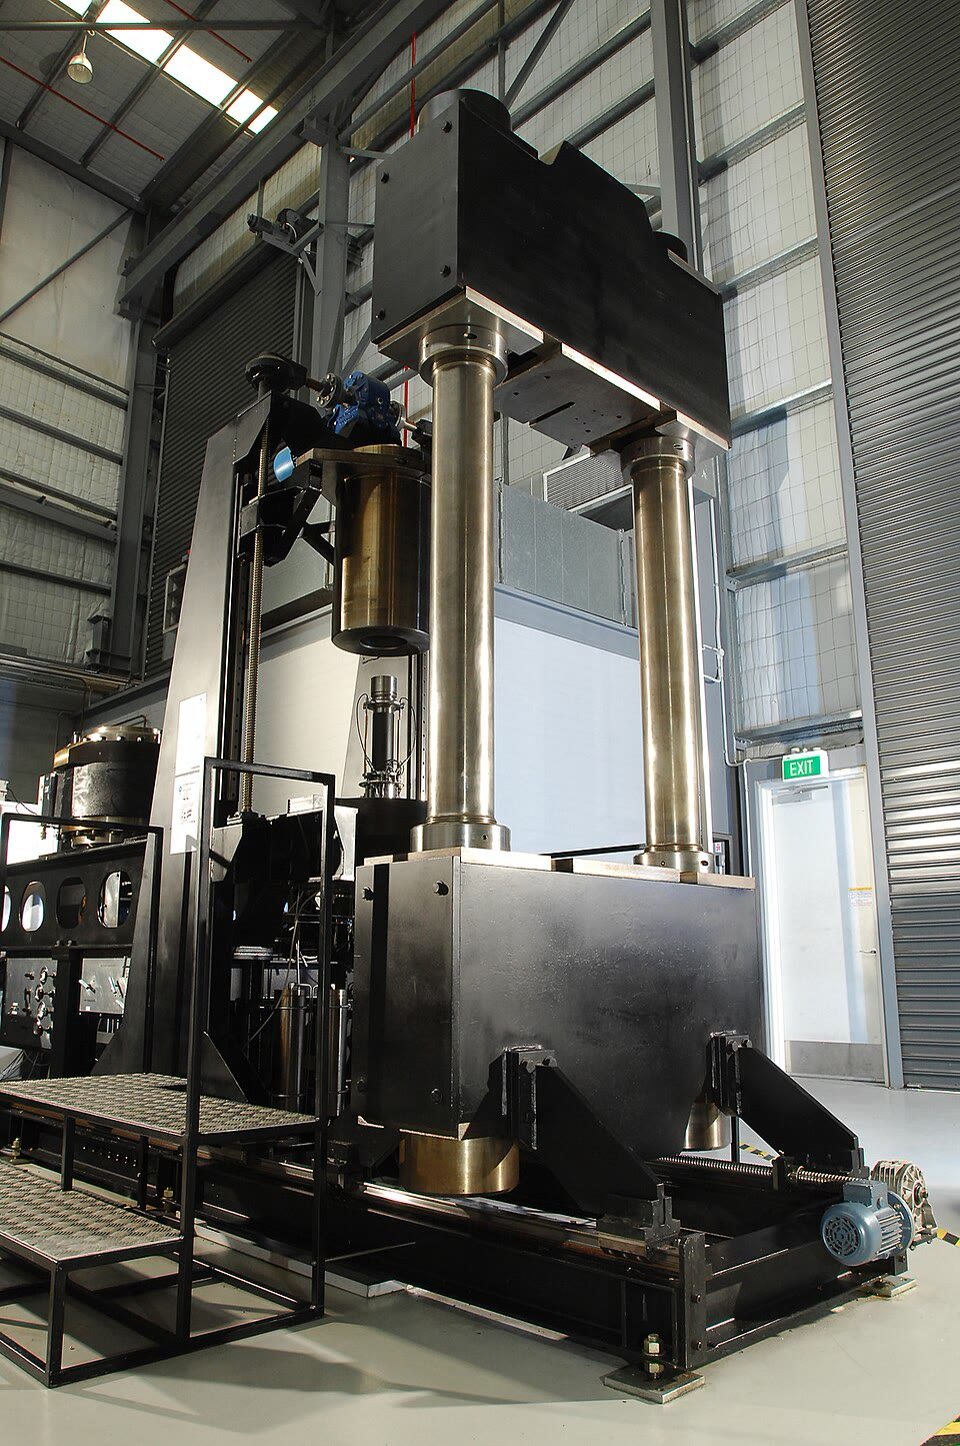
\includegraphics[width=\linewidth]{images/book3/b1-triaxial-cell.jpg}

{\scriptsize चट्टान की सामर्थ्य मापने के लिए एक उच्च-दाब त्रि-अक्षीय कक्ष (Darryl Peroni, CSIRO, CC BY 3.0)।}
% ledger: commons:csiro-triaxial
\end{minipage}
\end{inthelab}

\section{स्थलमंडल की सामर्थ्य}\label{sec:b1:stress-strain-rheology:envelope}

हर गहराई पर \omterm{def:b1:layered-earth:lithosphere}{स्थलमंडल} दो ढंगों से विफल हो सकता है: भ्रंशों पर फिसलकर, जिसकी सामर्थ्य प्रभावी दाब के साथ बढ़ती है, या विसर्पण से, जिसकी सामर्थ्य गरम होने पर घटती है। वह उस ढंग से विरूपित होता है जिसमें छोटा प्रतिबल चाहिए।

\begin{definition}[सामर्थ्य-आवरण, भंगुर–तन्य संक्रमण, भूकंप-जनक परत]
\label{def:b1:stress-strain-rheology:strength-envelope}
\omterm{def:b1:layered-earth:lithosphere}{स्थलमंडल} का \emph{सामर्थ्य-आवरण}\index{सामर्थ्य-आवरण} गहराई के विरुद्ध वह वक्र है जो दिए गए विकृति-दर पर वह अधिकतम \omterm{def:b1:stress-strain-rheology:principal}{अवकल प्रतिबल} दिखाता है जिसे वह सह सकता है: हर गहराई पर, घर्षण-सामर्थ्य और विसर्पण-सामर्थ्य में छोटी। \emph{भंगुर–तन्य संक्रमण}\index{भंगुर–तन्य संक्रमण} वह गहराई है जिस पर दोनों बराबर हैं: उसके ऊपर चट्टान भ्रंशन से विरूपित होती है, नीचे विसर्पण से। \emph{भूकंप-जनक परत}\index{भूकंप-जनक परत} गहराइयों का वह परास है जिसमें अधिकांश भूकंप शुरू होते हैं।
\end{definition}

\begin{proposition}[गहराई के साथ घर्षण-सामर्थ्य]
\label{prop:b1:stress-strain-rheology:brittle-gradient}
घनत्व $\rho$ की परत में, स्थैतिक छिद्र-दाब के साथ, जिसमें एक \omterm{def:b1:stress-strain-rheology:principal}{मुख्य प्रतिबल} ऊर्ध्वाधर है, हर दिशा के भ्रंश हैं और \omterm{def:b1:stress-strain-rheology:coulomb}{संसंजन} नहीं, घर्षण $\mu$ के साथ फिसलना \omterm{def:b1:stress-strain-rheology:principal}{अवकल प्रतिबल} पर शुरू होता है
\begin{align*}
  \sigma_1 - \sigma_3 &= \frac{2\mu}{\sqrt{1+\mu^2} + \mu}\,\rho g z(1-\lambda)
  && \text{यदि $\sigma_v = \sigma_1$}, \\
  \sigma_1 - \sigma_3 &= \frac{2\mu}{\sqrt{1+\mu^2} - \mu}\,\rho g z(1-\lambda)
  && \text{यदि $\sigma_v = \sigma_3$},
\end{align*}
जहाँ $\lambda = \rho_w/\rho$: पहली स्थिति सामान्य भ्रंश देती है, दूसरी उत्क्षेप।
\end{proposition}

\begin{proof}
ऊर्ध्वाधर \omterm{def:b1:stress-strain-rheology:lithostatic}{प्रभावी प्रतिबल} $S = \rho g z - \rho_w g z = \rho g z(1-\lambda)$ है। $C = 0$ और $k = \sqrt{1+\mu^2}$ के साथ, \cref{thm:b1:stress-strain-rheology:failure-angle} कहता है कि एक भ्रंश तब फिसलता है जब $r = \mu c'/k$, जहाँ $r$ त्रिज्या और $c'$ प्रभावी मोर वृत्त का केंद्र है। यदि $\sigma_v = \sigma_1$, तो $\sigma_1' = S$ और $c' = S - r$, अतः $rk = \mu S - \mu r$ और $r = \mu S/(k+\mu)$। यदि $\sigma_v = \sigma_3$, तो $c' = S + r$ और $r = \mu S/(k-\mu)$। \omterm{def:b1:stress-strain-rheology:principal}{अवकल प्रतिबल} $2r$ है।
\end{proof}

$\mu = 0.85$ और $\rho = \qty{2700}{kg.m^{-3}}$ के साथ, $S$ प्रति किलोमीटर \qty{16.7}{MPa} बढ़ता है, और घर्षण-सामर्थ्य प्रति किलोमीटर \qty{13.1}{MPa} खिंचाव के अंतर्गत और \qty{61.3}{MPa} संपीड़न के अंतर्गत, लगभग पाँच गुना अधिक: \omterm{def:b1:layered-earth:layers}{भूपर्पटी} को खींचकर अलग करना उसे धकेलकर साथ लाने से कहीं आसान है। प्रभावी \omterm{def:b1:stress-strain-rheology:stress}{अभिलंब प्रतिबल} \qty{200}{MPa} से आगे \omterm{prop:b1:stress-strain-rheology:byerlee}{बायरली नियम} की ऊपरी शाखा लागू होती है, और संपीड़न में ढलान घटकर लगभग \qty{35}{MPa} प्रति किलोमीटर रह जाती है।
% computed in figdata/bachelor-1/strength_envelope.py (tested); ledger: byerlee:1975

\begin{omfigure}
\begin{tikzpicture}
\pgfplotsset{envaxis/.style={omrecord, omdepth, scale only axis, width=5.6cm, height=7.2cm,
  xmin=-1000, xmax=2500, ymin=0, ymax=80, xtick={-1000,0,1000,2000},
  ytick={0,10,...,80}, unbounded coords=jump,
  xlabel={अवकल प्रतिबल $\sigma_1-\sigma_3$ (MPa)},
  tick label style={font=\scriptsize}, label style={font=\small},
  scaled x ticks=false, xticklabel style={/pgf/number format/.cd, 1000 sep={\,}}}}
% computed in figdata/bachelor-1/strength_envelope.py; ledger: byerlee:1975, lopez:flow-laws, codata:R, prem:moho-average
\begin{axis}[envaxis, name=cont, ylabel={गहराई (km)}, title={\small (क) महाद्वीप, \qty{55}{mW.m^{-2}}}]
\addplot[fill=omLithGranite!45, draw=none] table[x=x, y=depth] {figdata/out/bachelor-1-strength_envelope-continental-outline.dat};
\addplot[omThm, line width=0.5pt, restrict x to domain=-1:2450] table[x=thrust, y=depth] {figdata/out/bachelor-1-strength_envelope-continental.dat};
\addplot[omThm, line width=0.5pt, restrict x to domain=-2450:1] table[x expr=-\thisrow{normal}, y=depth] {figdata/out/bachelor-1-strength_envelope-continental.dat};
\addplot[omDef, line width=0.5pt, restrict x to domain=-1:2450] table[x=ductile, y=depth] {figdata/out/bachelor-1-strength_envelope-continental.dat};
\addplot[omDef, line width=0.5pt, restrict x to domain=-2450:1] table[x expr=-\thisrow{ductile}, y=depth] {figdata/out/bachelor-1-strength_envelope-continental.dat};
\addplot[black, line width=1.0pt] table[x=x, y=depth] {figdata/out/bachelor-1-strength_envelope-continental-outline.dat};
\draw[black!60, dashed] (axis cs:-1000,35) -- (axis cs:2500,35);
\node[font=\scriptsize, anchor=south east] at (axis cs:2480,35) {मोहो};
\draw[black, densely dotted] (axis cs:0,0) -- (axis cs:0,80);
\draw[black!70] (axis cs:660,13.7) -- (axis cs:1700,18) node[anchor=north, font=\scriptsize, align=center, text=black] {संक्रमण\\ \qty{14}{km}};
\draw[black!70] (axis cs:1870,44.6) -- (axis cs:1950,53) node[anchor=north, font=\scriptsize, align=center, text=black] {प्रावार\\ संक्रमण};
\node[font=\scriptsize, anchor=north, omThm] at (axis cs:1500,3) {संपीड़न};
\node[font=\scriptsize, anchor=north, omThm] at (axis cs:-560,3) {खिंचाव};
\node[font=\scriptsize, anchor=west, omDef] at (axis cs:40,31) {गीला क्वार्ट्ज़};
\node[font=\scriptsize, anchor=west, omDef] at (axis cs:300,66) {शुष्क ओलिवीन};
\end{axis}
\begin{axis}[envaxis, at={(cont.east)}, anchor=west, xshift=0.6cm, yticklabels={}, title={\small (ख) महासागरीय तल, \qty{60}{Myr} पुराना}]
\addplot[fill=omLithBasalt!45, draw=none] table[x=x, y=depth] {figdata/out/bachelor-1-strength_envelope-oceanic-outline.dat};
\addplot[omThm, line width=0.5pt, restrict x to domain=-1:2450] table[x=thrust, y=depth] {figdata/out/bachelor-1-strength_envelope-oceanic.dat};
\addplot[omThm, line width=0.5pt, restrict x to domain=-2450:1] table[x expr=-\thisrow{normal}, y=depth] {figdata/out/bachelor-1-strength_envelope-oceanic.dat};
\addplot[omDef, line width=0.5pt, restrict x to domain=-1:2450] table[x=ductile, y=depth] {figdata/out/bachelor-1-strength_envelope-oceanic.dat};
\addplot[omDef, line width=0.5pt, restrict x to domain=-2450:1] table[x expr=-\thisrow{ductile}, y=depth] {figdata/out/bachelor-1-strength_envelope-oceanic.dat};
\addplot[black, line width=1.0pt] table[x=x, y=depth] {figdata/out/bachelor-1-strength_envelope-oceanic-outline.dat};
\draw[black, densely dotted] (axis cs:0,0) -- (axis cs:0,80);
\draw[black!70] (axis cs:2003,38.2) -- (axis cs:1900,50) node[anchor=north, font=\scriptsize, align=center, text=black] {संक्रमण\\ \qty{38}{km}};
\node[font=\scriptsize, anchor=west, omDef] at (axis cs:300,66) {शुष्क ओलिवीन};
\end{axis}
\end{tikzpicture}
\par\smallskip{\small विकृति-दर \qty{e-15}{s^{-1}} पर \omterm{def:b1:stress-strain-rheology:strength-envelope}{सामर्थ्य-आवरण}। लाल: हाइड्रोस्टैटिक छिद्र-दाब के साथ \omterm{prop:b1:stress-strain-rheology:byerlee}{बायरली नियम} से घर्षण-सामर्थ्य, संपीड़न के लिए (उत्क्षेप भ्रंशन, दाईं ओर) और खिंचाव के लिए (सामान्य भ्रंशन, बाईं ओर, ऋणात्मक खींचा गया); नीला: महाद्वीपीय \omterm{def:b1:layered-earth:layers}{भूपर्पटी} में गीले क्वार्ट्ज़ाइट की और \omterm{def:b1:layered-earth:layers}{प्रावार} में शुष्क \omterm{def:b1:rock-forming-minerals:groups}{ओलिवीन} की विसर्पण-सामर्थ्य; काली रूपरेखा और छायांकन: सामर्थ्य, हर गहराई पर दोनों में से छोटी। (क) महाद्वीप, जिसका \omterm{def:b1:heat-budget:heat-flow}{सतह-ऊष्मा-प्रवाह} \qty{55}{mW.m^{-2}} है और \omterm{def:b1:layered-earth:layers}{भूपर्पटी} \qty{35}{km} मोटी: ऊपरी \omterm{def:b1:layered-earth:layers}{भूपर्पटी} सबल, निचली \omterm{def:b1:layered-earth:layers}{भूपर्पटी} दुर्बल, सबसे ऊपरी \omterm{def:b1:layered-earth:layers}{प्रावार} सबल। (ख) महासागरीय तल \qty{60}{Myr} पुराना: संपीड़न में \qty{38}{km} मोटी एक एकल सबल परत।}
\label{fig:b1:stress-strain-rheology:envelope}
\end{omfigure}

ऊपर का चित्र दो स्थलमंडलों के लिए दोनों सामर्थ्यों को एक साथ रखता है। महाद्वीप का \cref{ch:b1:heat-budget} का \omterm{def:b1:heat-budget:geotherm}{जियोथर्म} है, जिसका \omterm{def:b1:heat-budget:heat-flow}{सतह-ऊष्मा-प्रवाह} \qty{55}{mW.m^{-2}} है, गीले क्वार्ट्ज़ाइट की \qty{35}{km} मोटी \omterm{def:b1:layered-earth:layers}{भूपर्पटी}, और नीचे शुष्क \omterm{def:b1:rock-forming-minerals:groups}{ओलिवीन}; महासागरीय तल \qty{60}{Myr} पुराना है, उसी अध्याय के अर्ध-अंतरिक्ष \omterm{def:b1:heat-budget:geotherm}{जियोथर्म} के साथ, और समुद्र-तल से नीचे \omterm{def:b1:rock-forming-minerals:groups}{ओलिवीन}। विकृति-दर \qty{e-15}{s^{-1}} है। \qty{35}{km} \omterm{def:b1:layered-earth:reference-model}{संदर्भ पृथ्वी मॉडल} (\cref{ch:b1:layered-earth}) में महाद्वीपों के नीचे \omterm{def:b1:layered-earth:discontinuity}{मोहो} की औसत गहराई है।
% ledger: prem:moho-average

महाद्वीप के नीचे \omterm{def:b1:stress-strain-rheology:strength-envelope}{भंगुर–तन्य संक्रमण} संपीड़न में \qty{13.7}{km} पर, \qty{249}{\degreeCelsius} पर, और खिंचाव में \qty{17.1}{km} पर आता है। गरम \omterm{def:b1:layered-earth:layers}{भूपर्पटी} उसे ऊपर लाती, ठंडी उसे नीचे धकेलती, क्योंकि विसर्पण-नियम दिए गए प्रतिबल पर केवल तापमान पर निर्भर है। यह संक्रमण \omterm{def:b1:layered-earth:layers}{भूपर्पटी} का सबसे सबल स्तर है। उसके नीचे सामर्थ्य ढह जाती है: \omterm{def:b1:layered-earth:discontinuity}{मोहो} पर, \qty{527}{\degreeCelsius} पर, क्वार्ट्ज़ाइट \qty{7.6}{MPa} के नीचे प्रवाहित होता है, जबकि उसी तापमान पर \omterm{def:b1:rock-forming-minerals:groups}{ओलिवीन} को लगभग \qty{30000}{MPa} चाहिए होंगे, घर्षण-सामर्थ्य से इतने दूर कि \omterm{def:b1:layered-earth:layers}{प्रावार} का ऊपरी भाग फिर भंगुर है। दूसरा संक्रमण संपीड़न में \qty{44.6}{km} पर आता है। इस मॉडल की निचली \omterm{def:b1:layered-earth:layers}{भूपर्पटी} दो सबल परतों के बीच एक मुलायम परत है: ``जेली सैंडविच''। महासागर के नीचे पूरा \omterm{def:b1:layered-earth:lithosphere}{स्थलमंडल} \omterm{def:b1:rock-forming-minerals:groups}{ओलिवीन} है, और सामर्थ्य एक ही संक्रमण तक नीचे बढ़ती है, \qty{38.2}{km} पर, \qty{641}{\degreeCelsius} पर।
% computed in figdata/bachelor-1/strength_envelope.py (tested)

भूकंप महासागरीय आवरण से मेल खाते हैं: महासागरीय प्लेटों के भीतर, वे ऐसी गहराइयों तक पहुँचते हैं जहाँ तापमान \qtyrange{600}{800}{\degreeCelsius} है, मॉडल के एकल संक्रमण के \qty{641}{\degreeCelsius} के निकट। इससे गहरे भूकंप केवल वहाँ होते हैं जहाँ एक प्लेट दूसरी के नीचे धँसती है, \qty{700}{km} से अधिक गहराई तक (\cref{ch:b1:active-margins})।
% ledger: jackson:jelly, usgs:deepest

महाद्वीपीय \omterm{def:b1:layered-earth:layers}{प्रावार} पर तस्वीर विवादित है। लगभग बीस वर्षों तक जेली सैंडविच प्रचलित मत था, जो शुष्क \omterm{def:b1:rock-forming-minerals:groups}{ओलिवीन} के प्रयोगशाला-मापों और कुछ भूकंपों पर आधारित था, जिन्हें \omterm{def:b1:layered-earth:discontinuity}{मोहो} के नीचे माना गया था। 2002 में जेम्स जैक्सन ने तर्क दिया कि इसे छोड़ देना चाहिए: बेहतर गहराइयों ने दिखाया कि महाद्वीपों के भूकंप एक ही परत तक सीमित हैं, प्रायः ऊपरी \omterm{def:b1:layered-earth:layers}{भूपर्पटी}, कभी-कभी पूरी \omterm{def:b1:layered-earth:layers}{भूपर्पटी}, और नीचे \omterm{def:b1:layered-earth:layers}{प्रावार} में कोई विश्वसनीय भूकंप नहीं, भले ही \omterm{def:b1:layered-earth:discontinuity}{मोहो} केवल \qtyrange{300}{500}{\degreeCelsius} पर हो। \omterm{def:b1:rock-forming-minerals:groups}{ओलिवीन} में प्रति दस लाख भाग कुछ भाग जितना थोड़ा पानी उसे नाटकीय रूप से दुर्बल करने के लिए पर्याप्त है, और महाद्वीपीय \omterm{def:b1:layered-earth:layers}{प्रावार} में शायद उतना होता है; तब महाद्वीपों की सामर्थ्य मुख्यतः उनकी \omterm{def:b1:layered-earth:layers}{भूपर्पटी} में होगी। दोनों मत एक ही नियमों से भिन्न आवरण खींचते हैं, \omterm{def:b1:layered-earth:discontinuity}{मोहो} के नीचे शुष्क या गीले \omterm{def:b1:rock-forming-minerals:groups}{ओलिवीन} के साथ।
% ledger: jackson:jelly
कोई भी सही हो, आवरण एक सीमा है, माप नहीं: प्रयोगशाला के नियम विकृति-दर के कई परिमाण-क्रमों पर बहिर्वेशित किए जाते हैं, और वे जो चरम प्रतिबल दिखाते हैं, एक गिगापास्कल से अधिक, उन \qtyrange{1}{10}{MPa} से कहीं ऊपर हैं जिन्हें भूकंप मुक्त करते देखे जाते हैं।
% ledger: jackson:jelly

\section{अभ्यास}

\begin{exercise}[$\star$]\label{exo:b1:stress-strain-rheology:1}
\qty{2700}{kg.m^{-3}} घनत्व की \omterm{def:b1:layered-earth:layers}{भूपर्पटी} और $g = \qty{9.81}{m.s^{-2}}$ लीजिए। \qty{10}{km} की गहराई पर परिकलित कीजिए: (क) ऊर्ध्वाधर प्रतिबल, (ख) स्थैतिक छिद्र-दाब, (ग) ऊर्ध्वाधर \omterm{def:b1:stress-strain-rheology:lithostatic}{प्रभावी प्रतिबल} और छिद्र-दाब अनुपात $\lambda$।
\end{exercise}

\begin{exercise}[$\star$]\label{exo:b1:stress-strain-rheology:2}
(क) \qty{10}{km} लंबी एक परत \qty{13}{km} तक खिंचती है: उसका \omterm{def:b1:stress-strain-rheology:strain}{प्रसार} और उसका \omterm{def:b1:stress-strain-rheology:strain}{स्ट्रेच} दीजिए। (ख) एक और, \qty{10}{km} लंबी, \qty{7}{km} तक सिकुड़ती है। (ग) एक चट्टान की दो रेखाएँ जो लंबवत थीं, अब \ang{60} का कोण बनाती हैं: कोणीय कर्तन और \omterm{def:b1:stress-strain-rheology:strain}{कर्तन-विकृति} क्या हैं?
\end{exercise}

\begin{exercise}[$\star$]\label{exo:b1:stress-strain-rheology:3}
एक बिंदु पर, $\sigma_1 = \qty{100}{MPa}$ और $\sigma_3 = \qty{40}{MPa}$। (क) मोर वृत्त खींचिए। (ख) सबसे बड़ा कर्तन-प्रतिबल क्या है, वह किन तलों पर कार्य करता है, और उन पर कौन-सा \omterm{def:b1:stress-strain-rheology:stress}{अभिलंब प्रतिबल} कार्य करता है? (ग) उस तल पर $\sigma_n$ और $\tau$ परिकलित कीजिए जिसका अभिलंब $\sigma_1$ के साथ \ang{30} बनाता है।
\end{exercise}

\begin{exercise}[$\star$]\label{exo:b1:stress-strain-rheology:4}
एक चट्टान का \omterm{def:b1:stress-strain-rheology:coulomb}{संसंजन} \qty{10}{MPa} और \omterm{def:b1:stress-strain-rheology:coulomb}{आंतरिक घर्षण-कोण} \ang{30} है। (क) $\sigma_1$ से किस कोण पर वह टूटती है, और दो संभव भंग-तल एक-दूसरे से कौन-सा कोण बनाते हैं? (ख) $\sigma_3' = \qty{20}{MPa}$ के साथ, कौन-सा प्रभावी $\sigma_1'$ उसे तोड़ता है?
\end{exercise}

\begin{exercise}[$\star\star$]\label{exo:b1:stress-strain-rheology:5}
अक्ष $x$ (क्षैतिज) और $y$ (ऊर्ध्वाधर) में, $\sigma_{xx} = \qty{60}{MPa}$, $\sigma_{yy} = \qty{20}{MPa}$ और $\sigma_{xy} = \qty{15}{MPa}$। (क) \omterm{def:b1:stress-strain-rheology:principal}{मुख्य प्रतिबल} और कोण $\theta_p$ परिकलित कीजिए। (ख) \cref{prop:b1:stress-strain-rheology:transformation} से जाँचिए कि अभिलंब $\theta_p$ वाला तल कोई कर्तन-प्रतिबल नहीं वहन करता और \omterm{def:b1:stress-strain-rheology:stress}{अभिलंब प्रतिबल} $\sigma_1$ है। (ग) इस बिंदु पर सबसे बड़ा कर्तन-प्रतिबल क्या है?
\end{exercise}

\begin{exercise}[$\star\star$]\label{exo:b1:stress-strain-rheology:6}
एक कर्तन-क्षेत्र ने अपनी चट्टान को \omterm{def:b1:stress-strain-rheology:shear-types}{सरल कर्तन} $\gamma = 2$ से विरूपित किया है। (क) मुख्य \omterm{def:b1:stress-strain-rheology:strain}{स्ट्रेच} और \omterm{def:b1:stress-strain-rheology:strain-ellipse}{विकृति-दीर्घवृत्त} के लंबे अक्ष का कर्तन-दिशा से कोण परिकलित कीजिए। (ख) जाँचिए कि क्षेत्रफल नहीं बदला। (ग) पदार्थ की एक रेखा कर्तन-दिशा से \ang{45} पर थी, कर्तन की दिशा में उठती हुई: अब वह कहाँ है, और उसका \omterm{def:b1:stress-strain-rheology:strain}{स्ट्रेच} क्या है? (क) से तुलना कीजिए।
\end{exercise}

\begin{exercise}[$\star\star$]\label{exo:b1:stress-strain-rheology:7}
\qty{200}{m} मोटे एक कर्तन-क्षेत्र में, एक स्लेट के छोटे गोल धब्बे अक्षों के 4 से 1 अनुपात के दीर्घवृत्त बन गए हैं। \omterm{def:b1:stress-strain-rheology:shear-types}{सरल कर्तन} मानिए, क्षेत्रफल में कोई परिवर्तन नहीं। (क) $S_1$, $S_2$ और $\gamma$ ज्ञात कीजिए। (ख) क्षेत्र की दीवारों से किस कोण पर लंबे अक्ष होने चाहिए? (ग) एक दीवार दूसरी के आगे कितनी दूर खिसक गई है?
\end{exercise}

\begin{exercise}[$\star\star$]\label{exo:b1:stress-strain-rheology:8}
\qty{3}{km} की गहराई पर एक भ्रंश, \qty{2700}{kg.m^{-3}} घनत्व की \omterm{def:b1:layered-earth:layers}{भूपर्पटी} में, \omterm{def:b1:stress-strain-rheology:stress}{अभिलंब प्रतिबल} \qty{70}{MPa} और कर्तन-प्रतिबल \qty{30}{MPa} वहन करता है। (क) स्थैतिक छिद्र-दाब के साथ, क्या वह \omterm{prop:b1:stress-strain-rheology:byerlee}{बायरली नियम} के अनुसार फिसलता है? (ख) और यदि छिद्र बंद हों और $\lambda = 0.6$ हो? (ग) $\lambda$ का वह मान ज्ञात कीजिए जिस पर वह फिसलना शुरू करता है।
\end{exercise}

\begin{exercise}[$\star\star$]\label{exo:b1:stress-strain-rheology:9}
गीले क्वार्ट्ज़ाइट के विसर्पण-नियम का प्रयोग कीजिए (\cref{prop:b1:stress-strain-rheology:creep})। (क) उसे दस गुना तेज़ बहाने के लिए प्रतिबल किस गुणक से बढ़ना होगा? (ख) समान दर पर और $V = 0$ के साथ, \qty{400}{\degreeCelsius} और \qty{500}{\degreeCelsius} के बीच उसकी सामर्थ्य किस गुणक से घटती है? (ग) इन दोनों परिणामों से समझाइए कि \omterm{def:b1:stress-strain-rheology:strength-envelope}{भंगुर–तन्य संक्रमण} की गहराई विकृति-दर पर उतनी नहीं जितनी \omterm{def:b1:heat-budget:geotherm}{जियोथर्म} पर क्यों निर्भर करती है।
\end{exercise}

\begin{exercise}[$\star\star\star$]\label{exo:b1:stress-strain-rheology:10}
जहाँ ऊर्ध्वाधर प्रतिबल $\sigma_2$ है, भ्रंश स्ट्राइक-स्लिप हैं। मान लीजिए कि ऊर्ध्वाधर \omterm{def:b1:stress-strain-rheology:lithostatic}{प्रभावी प्रतिबल} तब माध्य $(\sigma_1' + \sigma_3')/2$ है। (क) दिखाइए कि संसंजन-रहित घर्षण $\mu$ के साथ फिसलना $\sigma_1 - \sigma_3 = 2\mu\,\rho g z(1-\lambda)/\sqrt{1+\mu^2}$ पर शुरू होता है। (ख) $\mu = 0.85$ और $\rho = \qty{2700}{kg.m^{-3}}$ के लिए मेगापास्कल प्रति किलोमीटर में ढलान परिकलित कीजिए, और उसे सामान्य और उत्क्षेप भ्रंशन की ढलानों के बीच रखिए। (ग) तीनों ढलानों में से हर एक को ऊर्ध्वाधर \omterm{def:b1:stress-strain-rheology:lithostatic}{प्रभावी प्रतिबल} के गुणक के रूप में व्यक्त कीजिए।
\end{exercise}

\begin{exercise}[$\star\star\star$]\label{exo:b1:stress-strain-rheology:11}
\qty{60}{Myr} पुराने महासागरीय \omterm{def:b1:layered-earth:lithosphere}{स्थलमंडल} को \qty{1350}{\degreeCelsius} से ठंडे हुए एक अर्ध-अंतरिक्ष के रूप में मॉडल कीजिए, सतह पर \qty{0}{\degreeCelsius} और $\kappa = \qty{e-6}{m^2.s^{-1}}$: $T = \num{1350}\operatorname{erf}\bigl(z/(2\sqrt{\kappa t})\bigr)$। (क) $2\sqrt{\kappa t}$ परिकलित कीजिए। (ख) \qty{600}{\degreeCelsius} और \qty{800}{\degreeCelsius} के समतापों की गहराइयाँ ज्ञात कीजिए। (ग) महासागरीय प्लेटों के भीतर के भूकंप वहाँ तक पहुँचते हैं जहाँ तापमान \qtyrange{600}{800}{\degreeCelsius} है। इस अध्याय की महासागरीय \omterm{def:b1:stress-strain-rheology:strength-envelope}{सामर्थ्य-आवरण} में \omterm{def:b1:stress-strain-rheology:strength-envelope}{भंगुर–तन्य संक्रमण} से, जो \qty{38.2}{km} और \qty{641}{\degreeCelsius} पर है, तुलना कीजिए।
% ledger: jackson:jelly
\end{exercise}

\begin{exercise}[$\star\star\star$]\label{exo:b1:stress-strain-rheology:12}
एक चट्टान को हर दिशा के भंग काटते हैं, सभी में $\sigma_2$ की दिशा है, \omterm{def:b1:stress-strain-rheology:coulomb}{संसंजन} नहीं और घर्षण 0.85। प्रभावी \omterm{def:b1:stress-strain-rheology:principal}{मुख्य प्रतिबल} $\sigma_1' = \qty{110}{MPa}$ और $\sigma_3' = \qty{20}{MPa}$ हैं। (क) दिखाइए कि कुछ भंग फिसलते हैं। (ख) फिसलने वाले भंगों और $\sigma_1$ के बीच कोण का परास ज्ञात कीजिए। परास के बीच में कौन-सा है? (ग) $\sigma_1'$ के किस मान तक, $\sigma_3'$ स्थिर रखते हुए, कम से कम एक भंग अब भी फिसलता है?
\end{exercise}

\section{समस्या: क्या भ्रंश फिसलेगा?}

\begin{problem}[{सप्ताहांत समस्या --- पाँच किलोमीटर की गहराई पर एक सामान्य भ्रंश पर प्रतिबल, उसका सुरक्षा-अंतर, और छिद्र-दाब में वह वृद्धि जो उसे फिसलाएगी}]
\label{pb:b1:stress-strain-rheology:1}
% values: calc/ch16.py; ledger: byerlee:1975, hb81:denver
एक भ्रंश उत्तर–दक्षिण \omterm{def:b1:geological-maps:attitude}{स्ट्राइक} करता है और पूर्व की ओर \ang{60} नत है। एक निपटान-कूप उसे \qty{5.00}{km} की गहराई पर पाता है, \qty{2700}{kg.m^{-3}} घनत्व की \omterm{def:b1:layered-earth:layers}{भूपर्पटी} में, जिसके छिद्र सतह से जुड़े हैं। कूप में एक माप भ्रंश के लंबवत क्षैतिज प्रतिबल \qty{75.0}{MPa} देता है; \omterm{def:b1:geological-maps:attitude}{स्ट्राइक} के अनुदिश क्षैतिज प्रतिबल उसके और ऊर्ध्वाधर प्रतिबल के बीच है, अतः समस्या ऊर्ध्वाधर पूर्व–पश्चिम तल में द्वि-आयामी है। $g = \qty{9.81}{m.s^{-2}}$, \qty{1000}{kg.m^{-3}} घनत्व का पानी और \omterm{prop:b1:stress-strain-rheology:byerlee}{बायरली नियम} लीजिए। प्रतिबल \qty{0.01}{MPa} तक दीजिए।

\medskip
\noindent\textbf{भाग I --- प्रतिबल की अवस्था।}
\begin{enumerate}
  \item भ्रंश की गहराई पर ऊर्ध्वाधर प्रतिबल परिकलित कीजिए।
  \item वहाँ स्थैतिक छिद्र-दाब और अनुपात $\lambda$ परिकलित कीजिए।
  \item दो प्रतिबलों में से कौन-सा $\sigma_1$ है और कौन-सा $\sigma_3$? प्रतिबल की यह अवस्था किस प्रकार का भ्रंश चलाती है?
  \item \omterm{def:b1:stress-strain-rheology:principal}{अवकल प्रतिबल}, मोर वृत्त का केंद्र और त्रिज्या परिकलित कीजिए।
  \item प्रभावी \omterm{def:b1:stress-strain-rheology:principal}{मुख्य प्रतिबल} और प्रभावी वृत्त का केंद्र परिकलित कीजिए।
  \item $x$ पूर्व की ओर क्षैतिज और $y$ ऊर्ध्वाधर मानकर, तीनों घटक $\sigma_{xx}$, $\sigma_{yy}$, $\sigma_{xy}$ लिखिए। $\sigma_{xy}$ शून्य क्यों है?
\end{enumerate}

\medskip
\noindent\textbf{भाग II --- भ्रंश पर प्रतिबल।}
\begin{enumerate}[resume]
  \item प्रश्न 6 के अक्षों में भ्रंश का इकाई अभिलंब, और उसका कोण $\theta$, $\sigma_1$ के साथ, दीजिए।
  \item \cref{prop:b1:stress-strain-rheology:transformation} से भ्रंश पर $\sigma_n$ और $\tau$ परिकलित कीजिए।
  \item मोर वृत्त से दोनों मान जाँचिए: $\sigma_1$ सिरे से किस कोण पर भ्रंश स्थित है?
  \item भ्रंश पर प्रभावी \omterm{def:b1:stress-strain-rheology:stress}{अभिलंब प्रतिबल} परिकलित कीजिए।
  \item अनुपात $\tau/\sigma_n'$ परिकलित कीजिए और उसकी 0.85 से तुलना कीजिए।
  \item वर्तमान प्रभावी \omterm{def:b1:stress-strain-rheology:stress}{अभिलंब प्रतिबल} के अंतर्गत कौन-सा कर्तन-प्रतिबल भ्रंश को फिसलाएगा? वह कितने मेगापास्कल कम है?
\end{enumerate}

\medskip
\noindent\textbf{भाग III --- मोर का वृत्त और बायरली नियम।}
\begin{enumerate}[resume]
  \item प्रभावी मोर वृत्त और बायरली रेखा को पैमाने पर खींचिए।
  \item वृत्त के केंद्र से रेखा तक की दूरी परिकलित कीजिए और उसकी त्रिज्या से तुलना कीजिए। क्या चट्टान से होकर कोई तल फिसल सकता है?
  \item कौन-सा तल पहले फिसलेगा? उसका $\sigma_1$ से कोण और उसकी \omterm{def:b1:geological-maps:attitude}{नति} दीजिए।
  \item \cref{prop:b1:stress-strain-rheology:brittle-gradient} से, वह \omterm{def:b1:stress-strain-rheology:principal}{अवकल प्रतिबल} परिकलित कीजिए जिस पर इस गहराई पर सामान्य भ्रंश फिसलते हैं, और उसे \qty{13.1}{MPa} प्रति किलोमीटर की ढलान से जाँचिए।
  \item सबसे अच्छी तरह उन्मुख तल के फिसलने के लिए क्षैतिज प्रतिबल को कितना नीचे गिरना होगा?
  \item इस समस्या के भ्रंश को फिसलने के लिए कितना नीचे? समझाइए कि वह नीचा क्यों है।
\end{enumerate}

\medskip
\noindent\textbf{भाग IV --- अंतःक्षेपण।}
\begin{enumerate}[resume]
  \item समझाइए कि छिद्र-दाब की वृद्धि $\Delta P$ प्रभावी वृत्त को बिना उसकी त्रिज्या बदले $\Delta P$ बाईं ओर खिसकाती है।
  \item सबसे अच्छी तरह उन्मुख तल को फिसलाने वाली छिद्र-दाब-वृद्धि परिकलित कीजिए।
  \item कूप पानी से भरा है। भ्रंश पर छिद्र-दाब को उस मात्रा से बढ़ाने के लिए पंप को कूप-मुख पर कितना अतिरिक्त दाब लगाना होगा? वह पानी के कितने ऊँचे स्तंभ के बराबर है?
  \item यदि भ्रंश पर घर्षण 0.85 के बजाय 0.6 होता, तो क्या वह पहले से फिसल रहा होता? भ्रंश की शांति उसके घर्षण के बारे में क्या कहती है?
  \item किस अनुपात $\lambda$ पर सबसे अच्छी तरह उन्मुख तल फिसलता है?
  \item मेगापास्कल में, एक दशमलव तक, छिद्र-दाब की कितनी वृद्धि इस भ्रंश को फिसलाती है?
\end{enumerate}
\end{problem}
